\documentclass{standalone}
\usepackage{tikz}
\usetikzlibrary{patterns, positioning}

\begin{document}
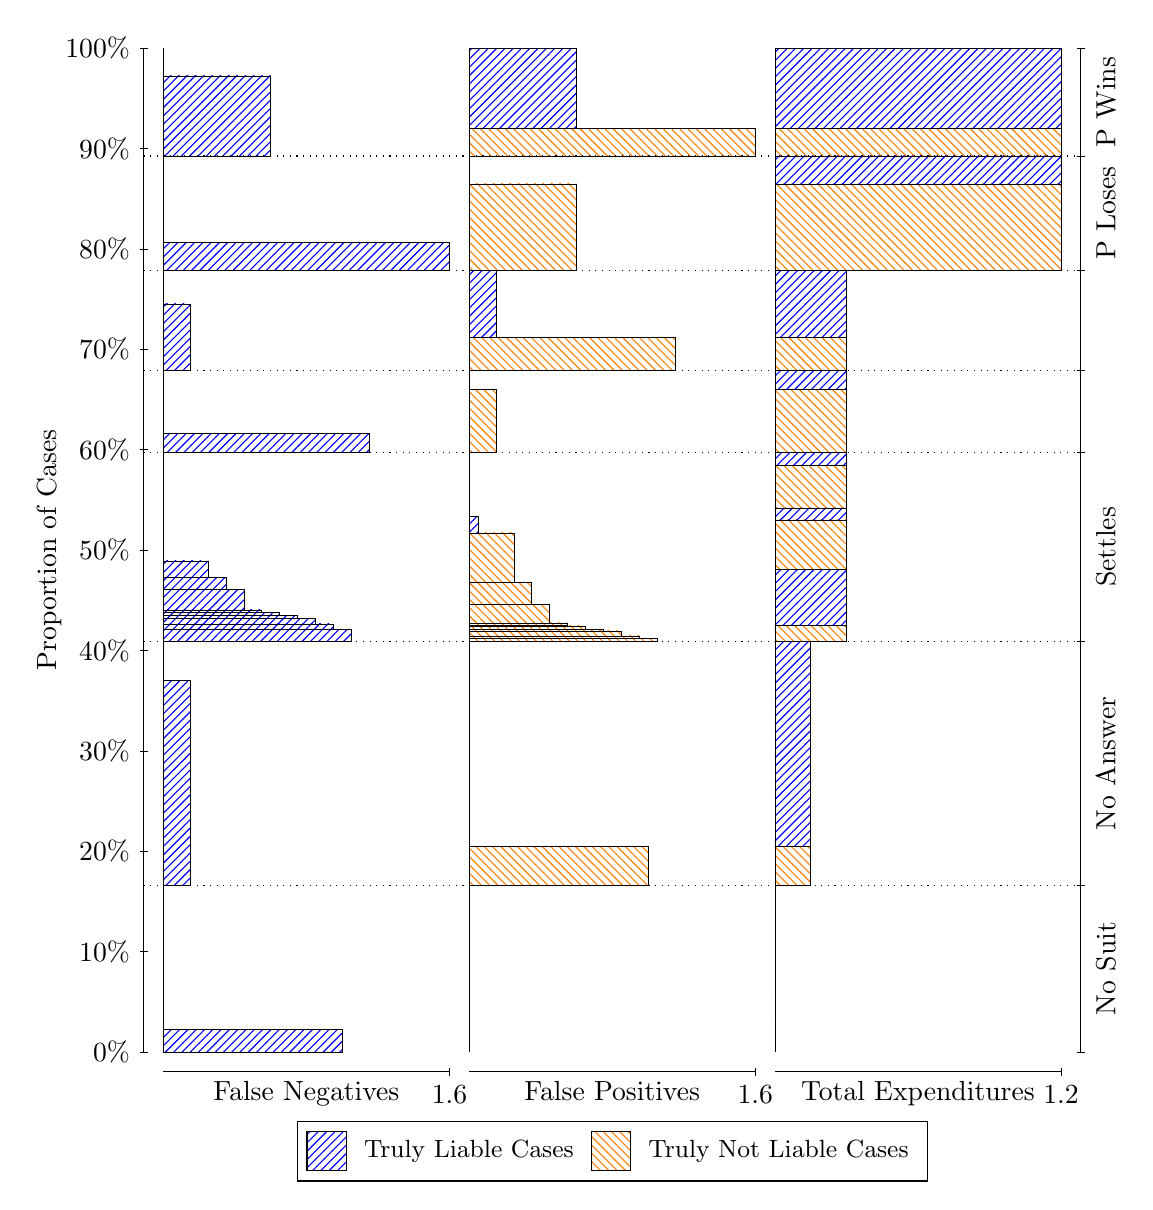
\begin{tikzpicture}
\draw[black, very thin] (1.5,1.75) -- (1.5,14.5);
\node[rotate=90, anchor=center] at (0.3, 8.125) {Proportion of Cases};
\draw[black, very thin] (1.45,1.75) -- (1.55,1.75);
\node[anchor=east] at (1.45, 1.75) {0\%};
\draw[black, very thin] (1.45,3.025) -- (1.55,3.025);
\node[anchor=east] at (1.45, 3.025) {10\%};
\draw[black, very thin] (1.45,4.3) -- (1.55,4.3);
\node[anchor=east] at (1.45, 4.3) {20\%};
\draw[black, very thin] (1.45,5.575) -- (1.55,5.575);
\node[anchor=east] at (1.45, 5.575) {30\%};
\draw[black, very thin] (1.45,6.85) -- (1.55,6.85);
\node[anchor=east] at (1.45, 6.85) {40\%};
\draw[black, very thin] (1.45,8.125) -- (1.55,8.125);
\node[anchor=east] at (1.45, 8.125) {50\%};
\draw[black, very thin] (1.45,9.4) -- (1.55,9.4);
\node[anchor=east] at (1.45, 9.4) {60\%};
\draw[black, very thin] (1.45,10.675) -- (1.55,10.675);
\node[anchor=east] at (1.45, 10.675) {70\%};
\draw[black, very thin] (1.45,11.95) -- (1.55,11.95);
\node[anchor=east] at (1.45, 11.95) {80\%};
\draw[black, very thin] (1.45,13.225) -- (1.55,13.225);
\node[anchor=east] at (1.45, 13.225) {90\%};
\draw[black, very thin] (1.45,14.5) -- (1.55,14.5);
\node[anchor=east] at (1.45, 14.5) {100\%};

\draw[black, very thin] (13.4,1.75) -- (13.4,14.5);
\draw[black, very thin] (13.35,1.75) -- (13.45,1.75);
\node[anchor=west] at (13.35, 1.75) {};
\draw[black, very thin] (13.35,3.8669) -- (13.45,3.8669);
\node[anchor=west] at (13.35, 3.8669) {};
\draw[black, very thin] (13.35,6.9619) -- (13.45,6.9619);
\node[anchor=west] at (13.35, 6.9619) {};
\draw[black, very thin] (13.35,9.3682) -- (13.45,9.3682);
\node[anchor=west] at (13.35, 9.3682) {};
\draw[black, very thin] (13.35,10.402) -- (13.45,10.402);
\node[anchor=west] at (13.35, 10.402) {};
\draw[black, very thin] (13.35,11.675) -- (13.45,11.675);
\node[anchor=west] at (13.35, 11.675) {};
\draw[black, very thin] (13.35,13.129) -- (13.45,13.129);
\node[anchor=west] at (13.35, 13.129) {};
\draw[black, very thin] (13.35,14.5) -- (13.45,14.5);
\node[anchor=west] at (13.35, 14.5) {};

\draw[black, very thin, pattern color=blue, pattern=north east lines] (1.75,1.75) rectangle (4.0208,2.0382);
\draw[black, very thin, pattern color=orange, pattern=north west lines] (1.75,2.0382) rectangle (1.75,3.8669);
\draw[black, very thin, pattern color=blue, pattern=north east lines] (1.75,3.8669) rectangle (2.0906,6.4643);
\draw[black, very thin, pattern color=orange, pattern=north west lines] (1.75,6.4643) rectangle (1.75,6.9619);
\draw[black, very thin, pattern color=blue, pattern=north east lines] (1.75,6.9619) rectangle (4.1344,7.1159);
\draw[black, very thin, pattern color=blue, pattern=north east lines] (1.75,7.1159) rectangle (3.9073,7.1862);
\draw[black, very thin, pattern color=blue, pattern=north east lines] (1.75,7.1862) rectangle (3.6802,7.253);
\draw[black, very thin, pattern color=blue, pattern=north east lines] (1.75,7.253) rectangle (3.4531,7.291);
\draw[black, very thin, pattern color=blue, pattern=north east lines] (1.75,7.291) rectangle (3.226,7.3366);
\draw[black, very thin, pattern color=blue, pattern=north east lines] (1.75,7.3366) rectangle (2.999,7.3636);
\draw[black, very thin, pattern color=blue, pattern=north east lines] (1.75,7.3636) rectangle (2.7719,7.6257);
\draw[black, very thin, pattern color=blue, pattern=north east lines] (1.75,7.6257) rectangle (2.5448,7.7739);
\draw[black, very thin, pattern color=blue, pattern=north east lines] (1.75,7.7739) rectangle (2.3177,7.9876);
\draw[black, very thin, pattern color=orange, pattern=north west lines] (1.75,7.9876) rectangle (1.75,9.3682);
\draw[black, very thin, pattern color=blue, pattern=north east lines] (1.75,9.3682) rectangle (4.3615,9.6104);
\draw[black, very thin, pattern color=orange, pattern=north west lines] (1.75,9.6104) rectangle (1.75,10.402);
\draw[black, very thin, pattern color=blue, pattern=north east lines] (1.75,10.402) rectangle (2.0906,11.252);
\draw[black, very thin, pattern color=orange, pattern=north west lines] (1.75,11.252) rectangle (1.75,11.675);
\draw[black, very thin, pattern color=blue, pattern=north east lines] (1.75,11.675) rectangle (5.3833,12.028);
\draw[black, very thin, pattern color=orange, pattern=north west lines] (1.75,12.028) rectangle (1.75,13.129);
\draw[black, very thin, pattern color=blue, pattern=north east lines] (1.75,13.129) rectangle (3.1125,14.147);
\draw[black, very thin, pattern color=orange, pattern=north west lines] (1.75,14.147) rectangle (1.75,14.5);
\draw[black, very thin, pattern color=orange, pattern=north west lines] (5.6333,1.75) rectangle (5.6333,3.5787);
\draw[black, very thin, pattern color=blue, pattern=north east lines] (5.6333,3.5787) rectangle (5.6333,3.8669);
\draw[black, very thin, pattern color=orange, pattern=north west lines] (5.6333,3.8669) rectangle (7.9042,4.3645);
\draw[black, very thin, pattern color=blue, pattern=north east lines] (5.6333,4.3645) rectangle (5.6333,6.9619);
\draw[black, very thin, pattern color=orange, pattern=north west lines] (5.6333,6.9619) rectangle (8.0177,7.0035);
\draw[black, very thin, pattern color=orange, pattern=north west lines] (5.6333,7.0035) rectangle (7.7906,7.0353);
\draw[black, very thin, pattern color=orange, pattern=north west lines] (5.6333,7.0353) rectangle (7.5635,7.0974);
\draw[black, very thin, pattern color=orange, pattern=north west lines] (5.6333,7.0974) rectangle (7.3365,7.1201);
\draw[black, very thin, pattern color=orange, pattern=north west lines] (5.6333,7.1201) rectangle (7.1094,7.1615);
\draw[black, very thin, pattern color=orange, pattern=north west lines] (5.6333,7.1615) rectangle (6.8823,7.1704);
\draw[black, very thin, pattern color=orange, pattern=north west lines] (5.6333,7.1704) rectangle (6.8823,7.1981);
\draw[black, very thin, pattern color=orange, pattern=north west lines] (5.6333,7.1981) rectangle (6.6552,7.4362);
\draw[black, very thin, pattern color=orange, pattern=north west lines] (5.6333,7.4362) rectangle (6.4281,7.711);
\draw[black, very thin, pattern color=orange, pattern=north west lines] (5.6333,7.711) rectangle (6.201,8.3425);
\draw[black, very thin, pattern color=blue, pattern=north east lines] (5.6333,8.3425) rectangle (5.7469,8.5563);
\draw[black, very thin, pattern color=blue, pattern=north east lines] (5.6333,8.5563) rectangle (5.6333,9.3682);
\draw[black, very thin, pattern color=orange, pattern=north west lines] (5.6333,9.3682) rectangle (5.974,10.16);
\draw[black, very thin, pattern color=blue, pattern=north east lines] (5.6333,10.16) rectangle (5.6333,10.402);
\draw[black, very thin, pattern color=orange, pattern=north west lines] (5.6333,10.402) rectangle (8.2448,10.825);
\draw[black, very thin, pattern color=blue, pattern=north east lines] (5.6333,10.825) rectangle (5.974,11.675);
\draw[black, very thin, pattern color=orange, pattern=north west lines] (5.6333,11.675) rectangle (6.9958,12.776);
\draw[black, very thin, pattern color=blue, pattern=north east lines] (5.6333,12.776) rectangle (5.6333,13.129);
\draw[black, very thin, pattern color=orange, pattern=north west lines] (5.6333,13.129) rectangle (9.2667,13.482);
\draw[black, very thin, pattern color=blue, pattern=north east lines] (5.6333,13.482) rectangle (6.9958,14.5);
\draw[black, very thin, pattern color=orange, pattern=north west lines] (9.5167,1.75) rectangle (9.5167,3.5787);
\draw[black, very thin, pattern color=blue, pattern=north east lines] (9.5167,3.5787) rectangle (9.5167,3.8669);
\draw[black, very thin, pattern color=orange, pattern=north west lines] (9.5167,3.8669) rectangle (9.9708,4.3645);
\draw[black, very thin, pattern color=blue, pattern=north east lines] (9.5167,4.3645) rectangle (9.9708,6.9619);
\draw[black, very thin, pattern color=orange, pattern=north west lines] (9.5167,6.9619) rectangle (10.425,7.1704);
\draw[black, very thin, pattern color=blue, pattern=north east lines] (9.5167,7.1704) rectangle (10.425,7.8757);
\draw[black, very thin, pattern color=orange, pattern=north west lines] (9.5167,7.8757) rectangle (10.425,8.5073);
\draw[black, very thin, pattern color=blue, pattern=north east lines] (9.5167,8.5073) rectangle (10.425,8.6612);
\draw[black, very thin, pattern color=orange, pattern=north west lines] (9.5167,8.6612) rectangle (10.425,9.2018);
\draw[black, very thin, pattern color=blue, pattern=north east lines] (9.5167,9.2018) rectangle (10.425,9.3682);
\draw[black, very thin, pattern color=orange, pattern=north west lines] (9.5167,9.3682) rectangle (10.425,10.16);
\draw[black, very thin, pattern color=blue, pattern=north east lines] (9.5167,10.16) rectangle (10.425,10.402);
\draw[black, very thin, pattern color=orange, pattern=north west lines] (9.5167,10.402) rectangle (10.425,10.825);
\draw[black, very thin, pattern color=blue, pattern=north east lines] (9.5167,10.825) rectangle (10.425,11.675);
\draw[black, very thin, pattern color=orange, pattern=north west lines] (9.5167,11.675) rectangle (13.15,12.776);
\draw[black, very thin, pattern color=blue, pattern=north east lines] (9.5167,12.776) rectangle (13.15,13.129);
\draw[black, very thin, pattern color=orange, pattern=north west lines] (9.5167,13.129) rectangle (13.15,13.482);
\draw[black, very thin, pattern color=blue, pattern=north east lines] (9.5167,13.482) rectangle (13.15,14.5);
\draw[black, dotted] (1.5,3.8669) -- (13.4,3.8669);
\draw[black, dotted] (1.5,6.9619) -- (13.4,6.9619);
\draw[black, dotted] (1.5,9.3682) -- (13.4,9.3682);
\draw[black, dotted] (1.5,10.402) -- (13.4,10.402);
\draw[black, dotted] (1.5,11.675) -- (13.4,11.675);
\draw[black, dotted] (1.5,13.129) -- (13.4,13.129);
\draw[black, very thin] (1.75,1.5) -- (5.3833,1.5);
\node[anchor=north] at (3.5667, 1.5) {False Negatives};
\draw[black, very thin] (5.3833,1.45) -- (5.3833,1.55);
\node[anchor=north] at (5.3833, 1.45) {1.6};

\draw[black, very thin] (5.6333,1.5) -- (9.2667,1.5);
\node[anchor=north] at (7.45, 1.5) {False Positives};
\draw[black, very thin] (9.2667,1.45) -- (9.2667,1.55);
\node[anchor=north] at (9.2667, 1.45) {1.6};

\draw[black, very thin] (9.5167,1.5) -- (13.15,1.5);
\node[anchor=north] at (11.333, 1.5) {Total Expenditures};
\draw[black, very thin] (13.15,1.45) -- (13.15,1.55);
\node[anchor=north] at (13.15, 1.45) {1.2};

\node[black, centered, rotate=90] at (13.72, 2.8085) {No Suit};
\node[black, centered, rotate=90] at (13.72, 5.4144) {No Answer};
\node[black, centered, rotate=90] at (13.72, 8.1651) {Settles};


\node[black, centered, rotate=90] at (13.72, 12.402) {P Loses};
\node[black, centered, rotate=90] at (13.72, 13.814) {P Wins};

\draw (7.449999999999999,1.5) node[draw=none] (baseCoordinate) {};
\begin{scope}[align=center]
        \matrix[scale=0.5, draw=black, below=0.5cm of baseCoordinate, nodes={draw}, column sep=0.1cm]{
            \node[rectangle, draw, minimum width=0.5cm, minimum height=0.5cm, pattern=north east lines, pattern color=blue] {}; &
            \node[draw=none, font=\small] (B) {Truly Liable Cases}; &
            \node[rectangle, draw, minimum width=0.5cm, minimum height=0.5cm, pattern=north west lines, pattern color=orange] {}; &
            \node[draw=none, font=\small] (B) {Truly Not Liable Cases}; \\
            };
\end{scope}

\end{tikzpicture}
\end{document}